%%%%%%%%%%%%%%%%%%%%%%%%%%%%%%%%%%%%%%%%%%%%%%%%%%%%%%%%%%%%%%%%%%%%%%
% nuthesis-template.tex - Miguel A, Lerma - 3/31/2013
%                         mlerma@math.northwestern.edu
%%%%%%%%%%%%%%%%%%%%%%%%%%%%%%%%%%%%%%%%%%%%%%%%%%%%%%%%%%%%%%%%%%%%%%

%%%%%%%%%%%%%%%%%%%%%%%% DISCLAIMER %%%%%%%%%%%%%%%%%%%%%%%%%%%%%%%%%%
% 
% In spite of the effort to accommodate this template and the nuthesis
% class to the official requirements of the university to write a 
% Ph.D. dissertation, it is not possible to guarantee that it will 
% always work, and the author of the dissertation remains responsible
% for checking that such requirements are actually fulfilled by 
% his/her final work.
%
%%%%%%%%%%%%%%%%%%%%%%%%%%%%%%%%%%%%%%%%%%%%%%%%%%%%%%%%%%%%%%%%%%%%%%


\documentclass[12pt]{nuthesis}	% The nuthesis class is based on 
				% amsbook.cls.
				
\usepackage[english]{babel}
\usepackage[utf8x]{inputenc}
\usepackage[T1]{fontenc}
\usepackage[natbibapa]{apacite}
\usepackage{comment}
\usepackage{todonotes}
\usepackage{graphicx}


%%%%%%%%%%%%%%%%%%%%%%%%%%%%%%%%%%%
% DATA OF AUTHOR AND DISSERTATION %
%%%%%%%%%%%%%%%%%%%%%%%%%%%%%%%%%%%

\author{Matthew Heston}

\title{The Effect of Contextual and Relational Variables on Predicting Mobile Responsiveness}

%\degree{DOCTOR OF PHILOSOPHY}  % Default: DOCTOR OF PHILOSOPHY

\field{Technology and Social Behavior}            % Default: Mathematics

%\graduationmonth{June}         % The default is June or December
                                % depending on current date.

%\graduationyear{2003}          % Default: current year.


				% Use \includeonly to select the 
%\includeonly{chap1,chap2,...}	% chapters to include if you are 
				% using the \include command below.
				% This way you can latex only a the 
				% part you are working on, which 
				% is faster than latexing the entire 
				% thesis. 


\begin{document}
%	
%	THE BODY OF YOUR THESIS STARTS HERE
%

%%%%%%%%%%%%%%%%%%%%%%
% Some initial stuff %
%%%%%%%%%%%%%%%%%%%%%%

\frontmatter		% Preliminary pages start here.

\maketitle		% Produces the title page.

\copyrightpage		% Creates the copyright page.


\abstract		% Abstract.

This is the abstract.

\acknowledgements	% Acknowledgements (optional).

Text for acknowledgments.

\preface		% Preface (optional).

This is the preface.


%% A few more optional pages (uncomment if needed)
%
\listofabbreviations
CMC --- Computer Mediated Communication \\
SIP --- Social Information Processing Theory \\
SIA --- Session Initiation Attempt
%
%This is the list of abbreviations (optional).
%
%\glossary
%
%This is the glossary (optional).
%
%\nomenclature
%
%This is the nomenclature (optional).
%
%% Note that the dedication text must be passed as an argument
%% of the \dedication command
%\dedication{This is the dedication (optional).}
%

\clearpage\phantomsection % needed for the hyperlinks to work correctly
\tableofcontents	% Table of Contents will be automatically
			% generated and placed here.

\clearpage\phantomsection % needed for the hyperlinks to work correctly
\listoftables		% List of Tables and List of Figures will be placed

\clearpage\phantomsection % needed for the hyperlinks to work correctly
\listoffigures		% here, if applicable (optional).



\mainmatter             % Actual text starts here.

%%%%%%%%%%%%%%%%%%%%%%%%%%%
% Actual text starts here %
%%%%%%%%%%%%%%%%%%%%%%%%%%%

% If there is an introduction it must be the first chapter

\chapter{Introduction}

~\citet{walther1992interpersonal} predicted that participants in text-based interaction such as email and instant messaging would find ways to adapt to these media, encoding and decoding relational cues in text and deriving psychological knowledge about one another. Although this broke from many other theories of computer-mediated communication (CMC) at the time which posited that the lack of various nonverbal cues in CMC meant such media were unsuitable for nuanced interpersonal communication and would only be used for unambiguous messages in organizations~\citep[e.g.][]{daft1986organizational,sproull1986reducing}, it is clear now that ~\citeauthor{walther1992interpersonal} was correct in his predictions. In addition to forming friendships with others they meet online~\citep{grinter2006chatting}, users also use CMC to maintain existing relationships~\citep{hu2004friendships}, and often develop more intimate relationships with those they communicate with in CMC due to increased self-disclosure~\citep{valkenburg2009effects}. Drawing on Walther's initial model, work since has focused on how users of these platforms encode relational information in text~\citep[e.g.][]{hancock2007expressing,pirzadeh2014you}.

Text-based interaction has become even more ubiquitous with the widespread adoption of mobile devices. A 2015 Pew Report found that 92\% of American adults own a cell phone, with 68\% of U.S. adults having a smart phone~\citep{anderson2015technology}. While smart phone users report using their device for a variety of reasons, such as following the news and finding local events, text messaging is the most widely used feature~\citep{smith2015us}, with other mobile messaging platforms such as WhatsApp and Kik becoming increasingly popular as well~\citep{duggan2015mobile}. Phone owners use text messaging to communicate with a variety of different types of contacts (e.g., friends, family, and co-workers) for a variety of different reasons, ranging from information seeking to simply ``killing time'' ~\citep{battestini2010large}. Many of the same used to signal emotional and relational information in instant messaging and email, such as emoticons and lexical choice, are used the same way in mobile messaging~\citep{lo2008nonverbal,tossell2012longitudinal}.

One cue that may be different in the mobile context is responsiveness, or the amount of time it takes to respond to a message. It has been suggested that responsiveness serves as a cue in CMC, with quick responses signaling immediacy, care, and presence~\citep{kalman2006pauses,walther1995nonverbal}. Indeed, responsiveness has been demonstrated to affect impressions. ~\citet{cramton2002attribution} discusses how long delays in email response are often misattributed, such that those waiting for a response view the slow responders as intentionally ignoring them. ~\citet{heston2017worth} found that short delays in instant messaging can cause a decrease in social attraction among individuals who know each other.

What makes responsiveness unique in mobile messaging is that users carry their devices with them nearly constantly. We know that this has created the expectation that users are constantly available and has increased expectations for immediate responses~\citep{church2013s}. We know less, however, about what actually affects how quickly users decide to respond in mobile messaging. It is possible, for example, that because they are aware of these expectations for fast responsiveness, users simply respond immediately whenever they are available to do so. There is evidence, however, that users consider their relationship with the person trying to reach them when deciding whether or not to respond~\citep{wohn2015ambient}. The content of a message may also matter, e.g., such that messages deemed more important by a recipient are more likely to get a quick response~\citep{dabbish2005understanding}.

It is likely that all of these factors -- a user's availability, their relationship with the person contacting them, and the content of the message -- affect responsiveness behavior, but no work to date has quantified the relative magnitudes of these different effects. Doing so has important theoretical consequences. If the primary driver of responsiveness is simply how available a user is (i.e., users always respond quickly so long as they are not busy), then we should dismiss the hypothesis that responsiveness is signal of intimacy in CMC, as suggested by ~\citet{kalman2006pauses} and ~\citet{walther1995nonverbal}. If, on the other hand, relational variables, such as how close the message recipient is to the message sender, have a large effect on response time, then responsiveness may be seen as carrying relational information in the same ways that other cues in CMC do.

Understanding what affects mobile responsiveness also has practical implications for the design of mobile text-based interaction platforms. HCI scholars have shown an interest in better supporting affective communication in mobile messaging platforms~\citep[e.g.][]{amin2005sensems}. With regards to responsiveness, recent work has suggested the design awareness displays, showing a message sender the predicted likelihood of getting a response from the person they are trying to contact, thus mitigating negative consequences associated with the expectations for a quick response~\citep{pielot2014didn}. If a user's availability is the main factor affecting whether or not they will respond, such a system might be reasonable. If, however, responsiveness is affected primarily by message content and sender-receiver relationship, such a system might not only be inaccurate, but also lack social nuance and cause other issues.

The goal of this dissertation is to quantify the effects of availability, message content, and sender-receiver relationship on mobile responsiveness. 

\chapter{Background}

\section{Cues in Computer-Mediated Communication}

Nonverbal communication is an essential part of how humans communicate, and includes a variety of elements such as appearance, touch, and proximity~\citep{burgoon2016nonverbal}. \todo[inline]{examples}

The lack of these nonverbal cues was central to early theoretical approaches to computer-mediated communication (CMC). Social Presence Theory~\citep{short1976social} described all media as fitting on a one-dimensional spectrum of \textit{social presence}, which refers to ``the degree of salience of the other person in an interaction''. Greater social presence was often tied directly to the nonverbal cues present in face-to-face (FtF) interaction~\citep[e.g.,][]{burgoon1984relational}, such that CMC, and especially text-based interaction, were thought to result in less social presence. It was also hypothesized that communicators would choose an appropriate medium for their message, e.g., avoid communicating potentially ambiguous message over a less rich medium given the higher likelihood of being misinterpreted~\citep{daft1986organizational}.

Such theories comprise what ~\citet{walther2002cues} refers to ``cues filtered out'' theories of CMC, so called because of their emphasis on the lack of nonverbal cues driving behavior. His own theory, Social Information Processing (SIP)~\citep{walther1992interpersonal}, rejects the notion that the lack of certain nonverbal cues restricts communicators' abilities. 

Conceptual models of social cognition in psychology described a ``social information processing'' system in which individuals decode various social stimuli about an interaction partner (e.g., physical traits and behaviors) over time to form a representation of the person~\citep{lord1985information}. This process was described as goal-motivated, or as \citet{wyer1980processing} describes, the focus of information processing changes depending on whether you just want to get to know someone or are deciding to take them out to dinner.\citeauthor{walther1992interpersonal} applied this model to CMC, assuming that communicators have the same motivations to form impressions of others in online environments. Rather than focusing on the lack of certain nonverbal cues or social stimuli such as physical traits, \citeauthor{walther1992interpersonal} noted that linguistic cues are also often used to convey relational information, such as form of address~\citep{argyle1976gaze} and other lexical choices~\citep{wiener1968language}. In addition to relying on these linguistic cues in CMC, he also noted the adoption of paralinguistic cues, such as emoticons, to convey emotion in CMC~\citep{carey1980paralanguage,sherblom1988direction}. In other words, whereas \citet{daft1986organizational} may suggest email is simply not appropriate for certain types of communication which may be thought of ambiguous, \citeauthor{walther1992interpersonal} would instead suggest email users adapt to the medium, encoding various cues to ensure a lack of ambiguity.

Early empirical work drawing on SIP focused on impression formation, i.e., individuals meeting each other in CMC environments and forming impressions over time~\citep[e.g.,][]{hancock2001impression,markey2002interpersonal,tanis2003social}. Nevertheless, as text-based communication platforms have become widely used not just for meeting others online, but for maintaining existing offline relationships~\citep{grinter2006chatting,pettegrew2015smart}, the same types of cues still are used to convey different types of information across different types of relationships~\citep{derks2008emoticons,pirzadeh2012expression}.

\subsection{Responsiveness}
SIP provides a useful conceptual framework to understand the role of responsiveness, or the time it takes for a communicator to respond to a message, in CMC. Timing has been demonstrated to be an important nonverbal element in FtF interaction~\citep{burgoon2016nonverbal}. \citet{mclaughlin1984conversation} details how different short gaps in conversation are a useful element of the turn-taking procedure, where speakers can interpret the gaps as a turn-allocation method. However, when a gap exceeds a certain limit, conversation partners may feel like conversation has broken down. In an experimental study, ~\citet{mclaughlin1982awkward} found that gaps of more than a few seconds led to conversation partners being rated as less competent conversationalists.

SIP posits that communicators are driven to refine their impressions of those they communicate with based on the cues available to them. In the same way that cues such as lexical choice~\citep{muir2017linguistic,nguyen2016effects} and emoticons~\citep{walther2001impacts} have been shown to affect impressions, responsiveness in CMC has also been linked to impressions. In an experimental study, \citet{kalman2011online} found that long delays in email response led to lower evaluations of job candidates by managers. In another experiment, \citet{heston2017worth} found that relatively small delays in instant messaging resulted in lower social attraction among friends.

Knowing that their communication partners decode these cues, communicators are also motivated to use such cues strategically to convey information. Emoticons, for example, have been linked to the desire to convey sarcasm in CMC~\citep{wolf2000emotional}. Although studies such as \citet{kalman2011online} and \citet{heston2017worth} have shown an effect of how responsiveness is ``decoded'' (i.e., in affecting impressions), no work has studied the ``encoding'' process, in other words, if communicators deliberately alter responsiveness behavior in order to convey relational information. However, it has been hypothesized that communicators do use responsiveness to convey feelings of intimacy and closeness~\citep{kalman2006pauses,walther1995nonverbal}.

\section{Mobile Devices and Perpetual Contact}

The adoption of mobile devices has had wide-reaching effects on the way we communicate. Notably, it allows for what scholars have called \textit{perpetual contact}~\citep{katz2002perpetual}: given that individuals now carry their cell phones with them nearly constantly, they are able to be in contact with others nearly constantly. This has afforded many new opportunities. \citet{ling200210} noted mobile devices' enabling of \textit{micro-coordination}, the ability to, for example, immediately inform someone if you're running a few minutes late for a meeting. The increasing use of mobile messaging~\citep{duggan2015mobile,smith2015us} has allowed young phone owners to use these platforms for relational maintenance purposes, staying in touch with both close friends and acquaintances~\citep{pettegrew2015smart}.

Although these examples demonstrate the utility of mobile devices, perpetual contact has also been associated with less desirable outcomes. Constant contact has been reported to increased feelings of anxiety, as friends may become overdependent as a result of constantly checking in with one another~\citep{baym2015personal}. \citet{ames2013managing} discusses how constant contact can be overwhelming and how users sometimes turn off their devices or turn on ``airplane mode'' in order to be unreachable.

\citet{hall2012calling} refer to this as a ``duality of interdependence.'' ~\citet{baxter1993relationship} discuss how relationship satisfaction and relationship maintenance behaviors are affected by various dialectical tensions including an autonomy---connection contradiction. ~\citeauthor{hall2012calling} argue that this tension is inherent to the increased access afforded by mobile phone technology.

HCI scholars have explored various ways of easing this tension through the design of communication platforms. In an experimental study, \citet{avrahami2007improving} found that by providing contextual information to a message sender about a message receiver, the senders were able to better time their messages as to not interrupt the receivers at an inappropriate time. A similar approach was suggested by \citet{pielot2014didn}, who developed a machine learning model to infer a receiver's likelihood of engaging with a received message in order to inform a message sender of the receiver's current availability.

Other work suggests availability should be considered more malleable. In a field study of cell phone use, \citet{grandhi2010technology} found that who sent a message and what the content of the message were more important in the decision to engage with it than the user's current availability. Interview participants in a study by \citet{wohn2015ambient} also described content and sender--receiver relationship to be important factors in deciding when to respond to a message.

\subsection{Responsiveness}

The studies above demonstrate many interacting factors which should affect responsiveness behavior in mobile messaging. \citet{bayer2015connection} argue that increased use of mobile devices has resulted in new normative expectations about constant connectivity. There is some empirical support this this proposition in \citet{church2013s}, whose interview participants reported expecting immediate response from those they contact on mobile messaging. This perspective does not contradict SIP --- users may still encode relational information through their responsiveness behavior --- but it does suggest that users' behavior may also be affected by these new expectations.

At the same time, interview participants across studies have expressed frustration with these expectations~\citep{ames2013managing}, and reported that relational and contextual factors are still the primary factors which affect their responsiveness behavior~\citep{grandhi2010technology,wohn2015ambient}, suggesting that fast responsiveness is not solely a response to new social norms.


\section{Relational Differences in Communication}




\chapter{The Current Project}

Responsiveness may be seen as a cue in the Social Information Processing theory of CMC. CMC scholars have suggested that fast responsiveness may be associated with immediacy and care in CMC \citep{kalman2006pauses,walther1995nonverbal}, and experimental studies have demonstrated that slow responsiveness across different text-based platforms can lead to negative evaluations~\citep{heston2017worth,kalman2011online}.

However, most cues that have been studied from a SIP perspective are explicitly encoded by a sender. Studies such as ~\citet{hancock2007expressing} and ~\citet{pirzadeh2012expression} focus on cues such as word choice, punctuation, and emoticons, all of which a message sender can choose to alter when writing a message. Responsiveness, on the other hand, may not always be a conscious choice, as an individual may not respond simply because he is busy. Responsiveness is affected by many different factors.

The first is likely simply the message receiver's availability. In addition to simply not having access to their device, ~\citet{avrahami2007improving} noted various situational factors that could affect a cell phone owner's decision to take a call, such as if they were currently with a group and would be soon as rude for leaving to accept the call. Even now as social norms shift and being on a phone to respond to a message may seem less inappropriate~\citep{rainie2015americans}, individual users likely have their own set of guidelines that govern a subjective sense of being available for incoming mobile messages.

If availability were the primary factor driving responsiveness behavior, responsiveness would represent a unique type of cue from a SIP perspective: one that is ``encoded'' almost entirely by external forces, but that nevertheless is decoded in a way that affects impressions of a conversation partner in CMC. Investigating the relationship between availability and responsiveness also provides a baseline to compare how important other factors are in affecting responsiveness. My first research question then is:

\textit{RQ1: What is the relationship between a user's current availability and their mobile responsiveness?}

Other factors may also affect responsiveness, however. From a turn-taking perspective of conversation~\citep{sacks1974simplest}, a participant in a conversation will know how to use his turn based on various cues from the previous turn. In mobile messaging, a user might decide to respond quickly based on certain attributes of a received message. For example, someone might be busy and not want to get involved in a text conversation, but nevertheless choose to respond right away to an request for information from someone, under the assumption that that will be the end of their exchange. Furthermore, certain cues in CMC have been associated with heightened urgency or immediacy~\citep{nguyen2014lexical}, which may cause a message receiver to respond more quickly. These effects may ``override'' a user's current availability, assuming they are available enough to see the message.

If these effects were strong, responsiveness more closely resembles the type of cues hypothesized by scholars such as ~\citet{walther1995nonverbal} and ~\citet{kalman2006pauses}, where the responsiveness behavior more closely resembles a deliberate choice made by a conversation participant in response to cues they perceive in a received message. My second research question is:

\textit{RQ2: What is the relationship between attributes of an incoming message, such as perceived urgency, and responsiveness? Is this relationship affected by a user's current availability?}

Finally, the relationship between a message sender and receiver could also affect responsiveness decisions. Work within social pragmatics has suggested various relational attributes that affect the conversation dynamics between parties~\citep{brown1987politeness,goldberg1990interrupting,west1979against,wolfson1990bulge}, and qualitative studies of mobile messaging have suggested social pressure can affect responsiveness behavior~\citep{church2013s}. In particular, the degree closeness between individuals, sometimes referred to as intimacy, along with status differences between individuals have been empirically shown to affect various nonverbal communication behaviors~\citep{guerrero1991waxing,henley1973power,leffler1982effects,sternglanz2004reading}.  At the same time, recent work has argued certain social pragmatic behavior that exists FtF is less important in CMC~\citep{schulze2017knowledge,stromer2015context}, so the relational attributes previously focused on by conversation analysts may not be as important in CMC, at least with regard to responsiveness decisions. In the same way as message-level attributes may ``override'' situational factors, the same may occur with these relational variables, i.e., a user may respond quickly to his boss even if he is busy because he feels pressure to seem available given their relationship.

Quantifying the effect of relational variables on responsiveness behavior will both allow us to see if the same relational attributes demonstrated to affect conversation behavior FtF also exists in CMC, as well as understand how responsiveness as a cue might vary based on relationship, building on work that has studied how other SIP cues change based on relational context~\citep[e.g.,][]{hancock2007expressing}. My final research question is:

\textit{RQ3: How do intimacy and status between a message sender and message receiver affect responsiveness? Is this effect affected by a user's current availability?}


\chapter{Methods}

\section{Participants}

\section{Procedure}

\subsection{Pre-Study Survey}

Recruitment materials directed participants to an initial survey, which was used to collect demographic information, information about how participants used their phones, as well as a personality assessment.

\subsubsection{Demographic Data}
\todo[inline]{Put demographics here.}

\subsubsection{Texting Use}
\todo[inline]{Put texting info here.}

\subsubsection{Personality Data}
Prior work has demonstrated a link between the ``Big 5'' personality traits~\citep{john1991big} and various mobile phone behaviors, including frequency of SMS use as well as responsiveness to SMS messages~\citep{chittaranjan2011s,de2013predicting,lepp2015exploring}, suggesting these traits may be a useful covariate to include in a responsiveness model. These traits were measured using a modified short version of the scale developed by \citet{rammstedt2007measuring}.
\todo[inline]{Put texting info here.}

\subsection{SMS Tracking Application}

After completing the pre-study survey, participants were emailed a link to a custom Android application developed to collect their text messages and experience sampling data when responding to messages. They were also provided with detailed instructions about the app and measures involved.

A background service monitored participants' SMS database, storing all messages sent and received during the study period on an external database, managed by Northwestern School of Communication IT. All sensitive information, including phone numbers and message content, were encrypted before being sent to the database. These encrypted values were also stored in the database to help ensure participant privacy. Multimedia content, such as photographs, were not stored. \todo[inline]{dyads}

The focus of this study is on responses to what ~\citet{avrahami2006responsiveness} call \textit{session initiation attempts} (SIA's). An SIA is any message that begins a new conversation session. Once users are engaged in a texting conversation, they tend to respond quickly~\citep{battestini2010large}, whereas we would expect more variation in responsiveness in deciding whether or not to engage with a conversation initiation.

An SIA is any incoming message that is received after some threshold of time has passed since the last interaction between the message sender and receiver. For example, if the threshold was set to one hour, in Figure 1, the incoming message that starts ``Hey, I don't want to wait...'' would be considered an SIA since days have passed since the last interaction, whereas the ``ok'' emoji would not, since only 11 minutes have passed.

\begin{figure}[h]
\centering
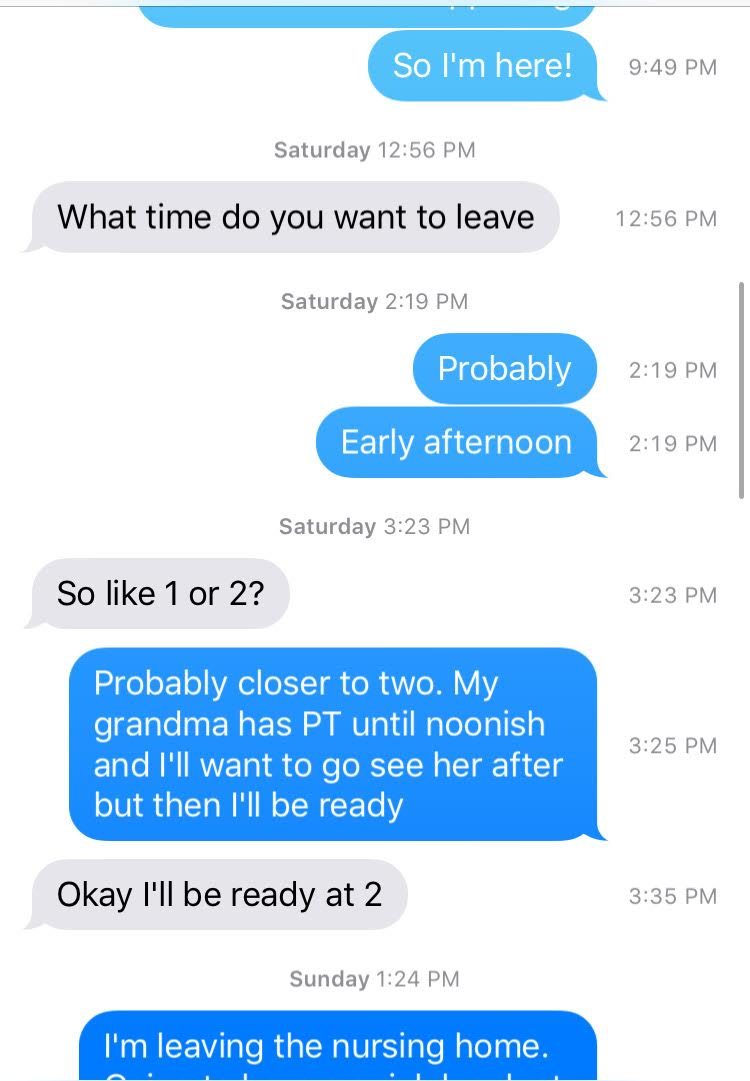
\includegraphics[width=.7\textwidth]{figures/example_sia}
\caption{Example text message exchange}
\end{figure}


\chapter{Discussion}

 \renewcommand\refname{\begin{centering}References\end{centering}}
 \bibliography{references.bib}
 \bibliographystyle{apacite} %or another suitable style.



% \appendix		% Appendix begins here (optional).

%\appendices	        % If more than one appendix chapters,
				% use appendices instead of appendix




\end{document}

